\documentclass{article}
\usepackage{ctex}
\usepackage[hidelinks]{hyperref}
\usepackage{appendix}
\usepackage{graphicx}
\usepackage{algorithm}
\usepackage{algpseudocode}
\title{AHashFlow实验方案}
\author{赵宗义}
\date{2019年11月13日}
\begin{document}
\maketitle

\tableofcontents

\section{基本定义}
\subsection{HashFlow}
原始的HashFlow方案,在数据平面记录完整的流标识符,没有控制平面,并且没有不活跃大流的退出机制。

\subsection{DHashFlow (HashFlow with Digest)}
在数据平面记录流标识符的摘要而不是完整的流标识符,同时增加控制平面来记录完整的流标识符,但是并没有引入不活跃大流的退出机制。在DHashFlow中,控制平面的作用仅仅是维护摘要和流标识符之间的映射关系,但是当有数据流从A表中升级到M表中而导致M表中的流数据项被替换的时候,我们并不会将被替换的流数据项导出至控制层。

\subsection{CHashFlow (HashFlow with Control Plane)}
CHashFlow基本上和DHashFlow类似,即包含了摘要映射机制以及和摘要映射机制相匹配的控制平面,但是CHashFlow比DHashFlow更进一步,因为在CHashFlow中当M表中的数据流因为A表中的数据流升级而被替换的时候我们并不会把它直接丢弃,而是会将它导出至控制平面。

\subsection{AHashFlow (Augmented HashFlow)}
这是我们最终版的改良方案,在数据平面记录流标识符的摘要而不是完整的流标识符,使用控制平面来维护流标识符和摘要之间的对应关系同时记录从控制平面导出的流记录项,此外还增加了不活跃大流的退出机制。

\section{测量指标}
假设我们重放的数据包序列中包含$m$个数据包和$n$个数据流,则相关的测量指标可以定义如下:

\subsection{包覆盖率 (PCR, Packet Covering Rate)}
假设我们的测量算法的M表记录的数据包的总数是$m'$,在CHashFlow和AHashFlow中则包括从M表导出到控制平面的数据包的数目,则测量算法的包覆盖率可定义如下:

$$
PCR = \frac{m'}{m}
$$

\subsection{数据包的不测量率  (NMR, No Measurement Rate)}
假设$m_1$是没有被我们的测量算法测量到数据包的数目,具体而言就是在辅助表中发生冲突的时候被丢弃的辅助表表项的计数值的总和,则数据包的不测量率可定义如下:
$$
NMR = \frac{m_1}{m}
$$

严格来说,HashFlow中M表中替换出去的包也不会被记录,因而属于不测量数据包的范畴,但是为了和包覆盖率相区别,我们在这里只计算没有机会被M表和A表记录的数据包,因为被M表和A表记录的数据包实际上是有可能通过控制层来记录的。

\subsection{ 流覆盖率(FSC, Flow Set Covering)}
假设网络测量算法记录了完整的流标识符的数目为$n_1$,则流覆盖率可定义如下:
$$
FSC = \frac{n_1}{n}
$$

\subsection{ 流数目估计相对误差(RE, Relative Error)}
假设网络测量算法估计的网络中数据流的数目为$n_2$,则流数目估计相对误差可定义如下:
$$
RE = \frac{|n - n_2|}{n}
$$

由于本文所考察的网络测量算法可以通过数据结构的使用情况估计没有被明确记录的数据流的数目,因此算法所估计的数据流数目和算法所明确记录的数据流的数目并不完全相等。

\subsection{ 数据流大小估计的平均相对误差(ARE, Average Relative Error)}
对于原数据包序列中的任意一个数据流$f_i$,假设它的真实大小为$m_i'$,而网络测量算法所返回的该数据流的大小为$m_i$,该数据流没有被测量算法明确记录则默认为$m_i'=0$,则数据流大小估计的平均相对误差可定义如下:
$$
ARE=\frac{1}{n}\sum\frac{|m_i - m'_i|}{m_i}
$$

\subsection{被测数据流大小估计的平均相对误差 (ARE, Average Relative Error)}
假设我们的测量算法记录的流分别为$f_1, f_2, ..., f_k$,且对于任意一个数据流$f_i ~(1 \le i \le k)$,它的实际大小为$m_i$,而我们的算法测得其大小为$m_i'$,则被测数据流大小估计的平均相对误差可定义为:
$$
ARE = \frac{1}{k}\sum\frac{|m_i - m'_i|}{m_i}
$$

\subsection{ heavy hitter检测的F1 Score}
已经定义heavy hitter的阈值$\gamma$,假设原数据包序列中heavy hitter的数目为$c_1$,网络测量算法所返回的heavy hitter的数目为$c_2$,网络测量算法所返回的heavy hitter中真实的heavy hitter的数目为$c$,则heavy hitter检测的召回率为$RR=\frac{c}{c_1}$,准确率为$PR=\frac{c}{c_2}$,因此heavy hitter检测的F1 Score可定义如下:
$$
F1~Score=\frac{2\cdot PR \cdot RR}{PR + RR}
$$

\subsection{ heavy hitter检测的平均相对误差(ARE, Average Relative Error)}
如上,假设原数据包序列中共有$n'$个heavy hitter,其中heavy hitter $f_i$的大小为$m_i$,而网络测量算法报告的$f_i$的大小为$m_i'$,如果$f_i$不包含在网络测量算法报告的heavy hitter中(包括$f_i$已经被网络测量算法记录但是没有被识别成为heavy hitter的情况),则默认$m_i'=0$,则heavy hitter检测的平均相对误差可定义如下:
$$
ARE = \frac{1}{n'}\sum\frac{|m_i - m'_i|}{m_i}
$$

\subsection{ 控制平面的包负荷比 (PLR, Packet Load Rate)}
在AHashFlow和DHashFlow中,我们需要将特定的信息(包括数据流的完整的流标识符以及主表中流记录)以数据包的形式从数据平面发送到控制平面以维护流标识符和指纹之间的映射关系,因此控制平面的包负荷比可定义如下:
$$
PLR = \frac{m_1}{m}
$$
其中$m_1$是控制平面处理的数据包的数目。

\subsection{控制平面的流负荷比 (PLR, Flow Load Rate)}
假设在AHashFlow(或DHashFlow)的运行过程中,控制平面一共收到了$m_1$个数据包,而交换机处理的数据包中一共包含了$n$个数据流,则控制平面的流负荷比可以定义如下:
$$
FLR = \frac{m_1}{n}
$$

\subsection{数据流的$x$-分布系数 ($x$ Distribution Coefficient)}
设$0<x<100$,对于某一个数据流,它的第一个数据包在trace文件中的序号为$a$,它的最后一个数据包在trace文件中的序号为$c$,数据流的$x\%$处的数据包在trace文件中的序号为$b$,则数据流的$x$-分布系数可定义为:
$$
xdc = \frac{b - a}{c - a}
$$

\section{实验设计}
\subsection{Exp84491 $\surd$}
\begin{itemize}
	\item Use the simulator of HashFlow implemented in python.
	\item Set the memory size to be 1 MB, so it can accommodate around 55K flow records.
	\item Select 10 trace files from each of the four traces.
	\item Initiate 50K flows from each trace file.
	\item Increase the depth of HashFlow from 1 to 4. 
	\item Count the packets processed by the simulator, i.e., the number of original packets plus the resubmitted packets.
\end{itemize}

\subsection{Exp84492 $\surd$}
\begin{itemize}
	\item Select a file from the CAIDA trace (equinix-nyc.dirA.20180315-125910.UTC.anon.pcap), extract the first 2.5 million packets, classify the TCP/UDP packets into flows, and then calculate the average size as well as the maximum size of the flows.
	\item Select a file from the HGC trace (20080415000.pcap), extract the first 2.5 million packets, classify the TCP/UDP packets into flows, and then calculate the average size as well as the maximum size of the flows.
	\item Calculate the average as well as maximum size of a file from China Telecom trace (nfcapd.201601022000).
	\item Calculate the average as well as maximum size of a file from Tsinghua campus trace (20140206-6). 
\end{itemize}

\subsection{Exp84493 $\surd$}
\begin{itemize}
	\item Set the memory size to be 1MB. 
	\item Increase the number of flows from 10K to 100K, in the step size of 10K.
	\item Use a trace file from CAIDA and HGC respectively.
	\item Use four versions of HashFlow. In the versions the number of buckets in the ancillary table is $0.25\times$, $0.5\times$, $1.0\times$, and $2\times$ respectively of the number of buckets in main table.
	\item Calculate the average relative error for flow size estimation.
\end{itemize}

\subsection{Exp84494 $\surd$}
\begin{itemize}
	\item Randomly select a file from the traces of ChinaTelecom, HGC, Tsinghua and CAIDA respectively. 
	\item Extract 5 million packets from each trace file.
	\item Record the number of distinct flows in each trace file. Note that all the packets with the same source IP address, destination IP address, source port, destination port, and protocol belong to the same flow. The flow ID is the five tuple (srcip, dstip, srcport, dstport, protocol).
	\item Map the flow ID of each flow to a digest using a given hash function.
	\item Record the number of distinct digest for each trace file. 
	\item Compare the number of distinct flows and the number of distinct digests for each trace file.
\end{itemize}

\subsection{Exp84495}
本实验的实验参数设置如下:
\begin{itemize}
\item 实验方案为HashFlow, DHashFlow和CHashFlow
\item 将内存容量设为1MB
\item 使用一个CAIDA的trace文件
\item 进行10组实验,将重放的数据包的数目以20万的步长从50万增加到250万
\item 将heavy hitter的阈值设为一个固定值10,即包含10个及10个以上数据包的流为一个heavy hitter
\item 测量的指标包括heavy hitters测量的F1 Score和平均相对误差,数据包的不测量率以及包覆盖率。
\end{itemize}

在此实验中可以预见的效果是,由于DHashFlow的M表比HashFlow的M表有更多的表项,因此DHashFlow的这四项性能指标都会明显优于HashFlow。同时,由于CHashFlow的控制层能够存储从数据层的M表中替换出来的流记录项,因此CHashFlow的heavy hitter检测的F1 Score和平均相对误差以及包覆盖率都会优于DHashFlow。此外,随着数据包数目的增加,各个算法的性能都会逐渐降低,但是HashFlow和DHashFlow的性能下降趋势相当,而CHashFlow的性能下降趋势要平缓得多。

\subsection{Exp84496}
本实验的实验参数设置如下:
\begin{itemize}
\item 实验方案为AHashFlow和CHashFlow
\item 将内存容量设为1MB
\item 从CAIDA和HGC的的trace中分别选取一个文件
\item 进行10组实验,将重放的数据包的数目以50万的步长从50万增加到500万
\item 测量的指标包括流覆盖率,数据流大小估计的平均相对误差,被测数据流大小估计的平均相对误差,以及控制平面的流负荷比
\end{itemize}

在此实验中,我们预期的实验结果是AHashFlow的这四项指标都保持相对稳定的状态,其中被测数据流大小估计的相对误差要明显小于数据流大小估计的平均相对误差,而控制平面的流负荷比接近2.0甚至小于2.0;AHashFlow的各项性能指标应该都要优于CHashFlow,尤其是CHashFlow的控制平面流负荷比应该会高于AHashFlow的控制平面流负荷比,说明在CHashFlow中不活跃大浪占据了宝贵的内存空间,导致其它的流更频繁地被替换。

\subsection{Exp84497}
本实验的实验参数设置如下:
\begin{itemize}
\item 实验方案为AHashFlow和CHashFlow
\item 将内存容量设为1MB
\item 从CAIDA和HGC的trace中分别选取一个文件
\item 仅进行1组实验,将重放的数据包的数目设为500万
\item 将heavy hitter的阈值以5的步长从5增加到50
\item 测量的指标包括heavy hitter检测的平均相对误差以及F1 Score
\end{itemize}

在此实验中我们的预期实验结果是随着阈值的增加,heavy hitter检测的F1 Score和平均相对误差都有明显的改善,说明AHashFlow确实有得大流的测量,同时AHashFlow的性能总是优于CHashFlow。

\subsection{Exp84498}
在CAIDA和HGC的trace中分别选择一个文件并对前500万个数据包按数据流进行归类,之后遍历整个文件,计算在前500万个数据包中出现的流中没有被正常结束(即收到一个结束标志或者重置标志)的流所占的比例。

对于那些正常结束的流,计算它们的$x$-分布系数,其中$x$的值暂时设定为90,并绘制这些流的$x$-分布系数的CDF图。

我们预期的实验结果是有相当一部分的数据流不能正常结束,并且对于正常结束的流,它们的$x$-分布系数会远远大于$1.0-x\%$,说明一个流要等待很久才会被正常结束。

\appendix
\section*{附录}
\section{AHashFlow方案介绍}
AHashFlow的数据结构如图\ref{fig:ahashflow}所示,AHashFlow的数据结构包括三个表,分别是M表、A表和B表,其中M表中的第一个表项包括一个4字节的digest域和一个4字节的count域,A表中每个表项包括一个1字节的digest域和一个1字节的count域,B表中每个表项包含一个4个节的count域。
\begin{figure}[ht!]
	\centering
	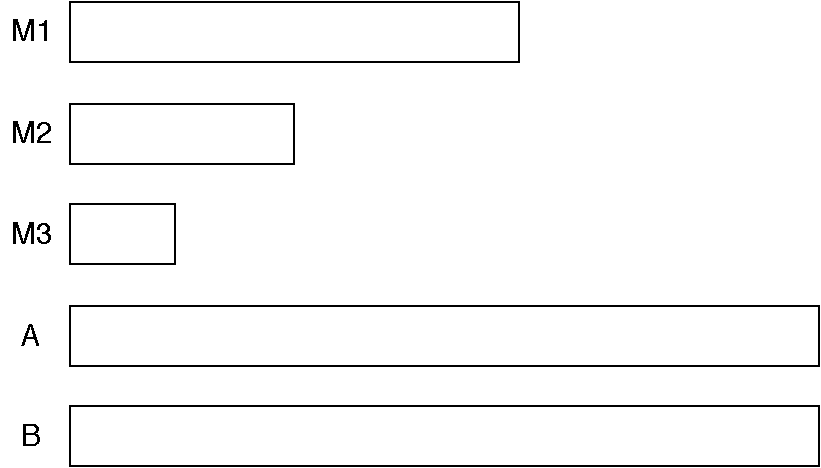
\includegraphics[width=0.7\linewidth]{./figures/AHashFlowDataStructure/AHashFlow}
	\caption{AHashFlow的数据结构:包括一个M表,一个A表以及一个B表,其中M表可分成若干小表}
	\label{fig:ahashflow}
\end{figure}

建议的内存分配方案是使得M表、A表和B表有相同数目的表项;M表可以分成若干个小表,其中后一个小表的表项数目是前一个小表的表项数目的一半。



\begin{algorithm}[ht!]
	\caption{$promote(idx, digest, cnt)$}
	\label{alg: promote}
	\begin{algorithmic}[1]
		\State{$export({\textbf A}[idx].digest, {\textbf A}[idx].cnt)$}
		\State{${\textbf A}[idx]\gets [digest, cnt]$}
	\end{algorithmic}
\end{algorithm}

\begin{algorithm}[ht!]
	\caption{$reset(idx)$}
	\label{alg: reset}
	\begin{algorithmic}[1]
		\State{$export({\textbf A}[idx].digest, {\textbf A}[idx].cnt)$}
		\State{${\textbf A}[idx].cnt\gets 0$}
	\end{algorithmic}
\end{algorithm}

\begin{algorithm}[ht!]
	\caption{$processPacket(p)$}
	\label{alg: processPacket}
	\algrenewcommand\algorithmicwhile{\textbf{when}}
	\begin{algorithmic}[1]
		\State{$min \gets \infty, max \gets 0, idx_{min} \gets -1, idx_{max}\gets -1$}
		\State{$digest_1\gets H_1(p.flowID), digest_2\gets H_2(p.flowID)$}
		\For{$i=1$ to $d$}
		\State{$idx\gets h_{i}(p.flowID)$}
		\If{${\mathbf M}[idx]== [0, 0]$}
		\State{${\mathbf M}[idx] \gets (digest_1, 1)$, $export(p.flowID)$}
		\Return
		\ElsIf {${\mathbf M}[idx].key == digest_1$}
		\State{Increment ${\mathbf M}[idx].cnt$ by 1}
		\Return
		\Else
		\If{${\mathbf M}[idx].count < min$}
		\State{$min \gets {\mathbf M}[idx].cnt, idx_{min}\gets idx$}
		\EndIf
		\If{${\mathbf M}[idx].count > max$}
		\State{$max\gets {\mathbf M}[idx].cnt, idx_{max}\gets idx$}
		\EndIf
		\EndIf
		\EndFor
		\State{$idx\gets g(p.flowID)$}
		\If{${\mathbf A}[idx] == [0, 0]$}
		\State{${\mathbf A}[idx] \gets [digest_2, 1]$}
		\ElsIf{${\mathbf A}[idx].key == digest_2$}
		\State{$temp \gets {\mathbf A}[idx].cnt + 1$}
		\If{$temp > min$}
		\State{$export(p.flowID)$, ${\mathbf A}[idx]\gets [0, 0]$}
		\State{$promote(idx_{min}, digest1, temp)$}
		\Else
		\State{${\mathbf A}[idx].count = temp$}
		\EndIf
		\Else
		\State{$temp \gets {\mathbf B}[idx].cnt + {\mathbf A}[idx].cnt$, ${\mathbf A}[idx] \gets [digest_2, 1]$}
		\If{$temp > max$}
		\State{$reset(idx_{max})$, ${\mathbf B}[idx] \gets 0$}
		\Else
		\State{${\mathbf B}[idx] \gets temp$}
		\EndIf
		\EndIf
	\end{algorithmic}
\end{algorithm}



AHashFlow对数据包的处理流程如算法\ref{alg: processPacket}所示,当一个数据包到达时,提取它的流标识符(默认为它的五元组(源IP地址,目的IP地址,源端口号,目的端口号,协议类型)),并将流标识符映射成为一个32位的$digest_1$和一个8位的$digest_2$。

之后,我们根据这个数据包的流标识符依次将这个数据包映射到M表的$d$个位置。在这$d$个位置上,如果我们找到了一个空表项,那么我们就将$digest_1$写入该表项中并将其计数值置为1,同时将数据包的流标识符导出到控制层,之后结束对数据包的处理。如果我们在M表中找到了一个digest域为$digest_1$的表项,那么我们只需要简单地将这个表项的计数值增加1便可以完成对这个数据包的处理。

反之,如果我们在这$d$个位置都不能找到一个空表项或者一个digest域的值为$digest_1$的表项,那么我们就记录这$d$个表项中的最大计数值$max$和最小计数值$min$,以及与之相对应的索引$idx_{max}$和$idx_{min}$。随后,我们进一步查询A表和B表。我们首先使用另一个哈希函数$g$将数据包的流标识符映射到一个索引值$idx$。由于A表和B表具有相同数目的表项,所以我们建议在A表和B表中均使用索引值$idx$。首先如果A表中对应的表项为空,则我们将该表项的内容设为$[digest_2, 1]$,于是便可以结束对数据包的处理。但是如果该表项不为空且它的digest和$digest_2$相同,那么我们就在A表中找到了一个匹配的表项,因此我们首先把这个表项的计数值加1并记录在一个临时变量$temp$中。如果$temp > min$,则说明A表中缓存的数据流比$min$对应的数据流更大,因此按照优先记录大流的原则 ,我们使用$promote$函数将这个流提回M表中。因为我们在M表中并不记录数据流的完整流标识符,因此我们需要将这个数据包的流标识符导出到控制层。最后我们再将A表中的这个表项置为空。如果$temp \le min$,则我们需要将$temp$写回到该表项的计数值中,实际上是将这个计数值加1。

如果该表项的计数值不为空且它的digest和$digest_2$不相同,说明新到达的数据包和A表中的相应表项发生冲突,那么我们首先将A表中相应表项的计数值和B表中$idx$对应的表项的计数值相加并存入$temp$中,然后再将A表中$idx$对应的表项置为$[digest_2, 1]$。随后我们比较$temp$和$max$的大小。因为M表和B表具有相同的表项数目,而且M表优先记录大流,而被B表记录的数据包一般来自小流,已知在正常的网络中绝大多数的数据包都来自大流,因此M表中表项的计数值应该远大于B表中表项的记数值。于是,如果$temp>max$,那么我们就断定测量算法的性能已经下降到一个需要引起注意的程度。而测量算法的性能下降的一个最重要的原因就是主表中表项已经被不活跃的大流占据,从而使得很多其它的流不能有效地在M表中积累。这里我们怀疑$max$对应的流是一个不活跃的大流,因此我们引入不活跃大流退出机制,将M表中$idx_{max}$对应的表项进行重置,同时将$idx$对应的B表的表项置为0。反之,如果$temp <= max$,则我们只需要简单将$temp$的值写入$idx$对应的B表表项中,相当于将该表项加1。


以下我们描述$promote$和$reset$两个算法即算法\ref{alg: promote}和\ref{alg: reset}的算法操作及其逻辑。首先在$promote$中,我们的参数包括一个索引值$idx$,新数据流的流标识符的digest以及对应的计数值。我们在主表中找到$idx$对应的表项并将其导出到控制层,然后将新数据流的digest和计数值写入到$idx$对应的主表表项中。而在$reset$中,我们的参数是主表中待重置表项的索引值$idx$,因此我们找到$idx$对应的主表表项并将其导出到控制层。此后,我们将该表项的计数值置为0,但是并不会对它的digest进行更改(即并不会将该表项的digest域也置为0),这样的方案设计主要是出于两个方面的原因的考虑。首先如果我们将$idx$对应的表项都置为空,那么M表中就可能出现一个数据流存放在多个表项中的情况,比如我们在图\ref{fig:ahashflow}中将$M1$中的一个表项$M1[x]$置为空,另一个流$f$会被映射到$M1$和$M2$中的两个表项$M1[x]$和$M2[y]$且我们已经为$f$在$M2[y]$维护了一个流表项,那么$f$的下一个数据包到达的时候我们检测到$M1[x]$为空,因此还会在$M1[x]$为它建立一个流表项,这样我们在M表中就为$f$维护了重复的流表项,造成了内存资源的浪费。如果我们只是将$M1[x]$的计数值置为0而保留它的digest就可以完美避开这个问题。此外,因为主表中被重置的流是一个大流,并且我们不能完全确定它是一个不活跃的大流,相反,它有可能是一个非常活跃的大流,因此我们仍然为它在主表中保留一个表项,如果它真的是一个活跃大流的话它就可以迅速在这个表项中聚集起来,避免了在A表中积累最后被$promote$的过程,可以有效减少测量误差。
\end{document}

